\documentclass{article}

% Text layout
\topmargin 0.0cm
\oddsidemargin 1cm
\evensidemargin 1cm
\textwidth 17cm 
\textheight 24cm

\usepackage{Sweave}
\begin{document}
\Sconcordance{concordance:L1.tex:L1.Rnw:%
1 9 1 1 0 2 1 1 14 13 0 1 4 3 0 1 7 6 0 1 2 2 1 1 2 1 0 1 1 1 7 5 0 1 1 %
4 0 1 2 1 5 4 0 1 8 7 0 1 2 2 1 1 2 1 0 1 1 1 6 4 0 1 1 4 0 1 2 1 5 4 0 %
1 8 7 0 1 2 2 1 1 2 1 0 1 1 1 6 4 0 1 1 4 0 1 2 1 5 4 0 1 7 6 0 3 1 1 2 %
1 0 1 1 1 5 4 0 1 1 4 0 1 2 1 5 4 0 1 7 6 0 1 2 2 1 1 2 1 0 1 1 1 2 1 3 %
2 0 1 1 4 0 1 2 1 5 4 0 1 9 8 0 1 2 3 1 1 3 1 0 1 2 1 0 1 1 1 3 1 0 1 1 %
1 7 5 0 1 1 4 0 1 2 1 5 4 0 1 8 7 0 1 2 2 1 1 2 1 0 2 1 1 5 4 0 1 2 5 0 %
1 2 1 5 4 0 1 6 5 0 1 2 1 1 2 2 1 0 1 1 1 6 4 0 1 1 4 0 1 2 1 5 4 0 1 6 %
5 0 1 2 1 1 1 3 1 11 10 0 1 1 4 0 1 2 1 5 4 0 1 15 14 0 1 2 3 1 1 3 1 0 %
1 2 1 0 1 1 1 2 1 7 5 0 1 2 5 0 1 2 1 1}

\setkeys{Gin}{width=0.35\textwidth}
\begin{Schunk}
\begin{Sinput}
> #  PROJECT 
> #  =======
> #  Principles of Modelling and Simulation in Epidemiology
> #  Laboratory exercise 1
> #
> #  DESCRIPTION
> #  ===========
> #  Suggestions of solutions
> 
> # AUTHOR AND DATE
> # Andreas Karlsson, October 2013
> 
> require(deSolve)
> ## =============================================================================
> ## 2.1 Filling and draining compartments
> ## =============================================================================
> rm(list=ls(all=TRUE)) 
> deriv <- function(time, state, parameters) {
+   with(as.list(c(state, parameters)), {
+     dX1 <- c1 - c2
+     dX2 <- c2 - c1
+     return(list(c(dX1, dX2)))
+   })
+ }
> init <- c(X1 = 17.3, X2 = 0)
> parameters <- c(c1 = 10, c2 = 5)
> times <- seq(0, 10, by = 0.01)
> out <- as.data.frame(ode(y = init, times = times, func = deriv, 
+                          parms = parameters))
> out$time <- NULL
> ##-----------------------------
> ## Plot results
> ##-----------------------------
> matplot(times, out, type = 'l', xlab = 'Time', ylab = 'AU', 
+         main = 'Dispersion of a flow that passes a dynamic structure', 
+         lty = 1, bty = 'l', col = 2:3)
> legend('topleft', c('5*t','-5*t'), lty = 1, col = 2:3)
\end{Sinput}
\end{Schunk}
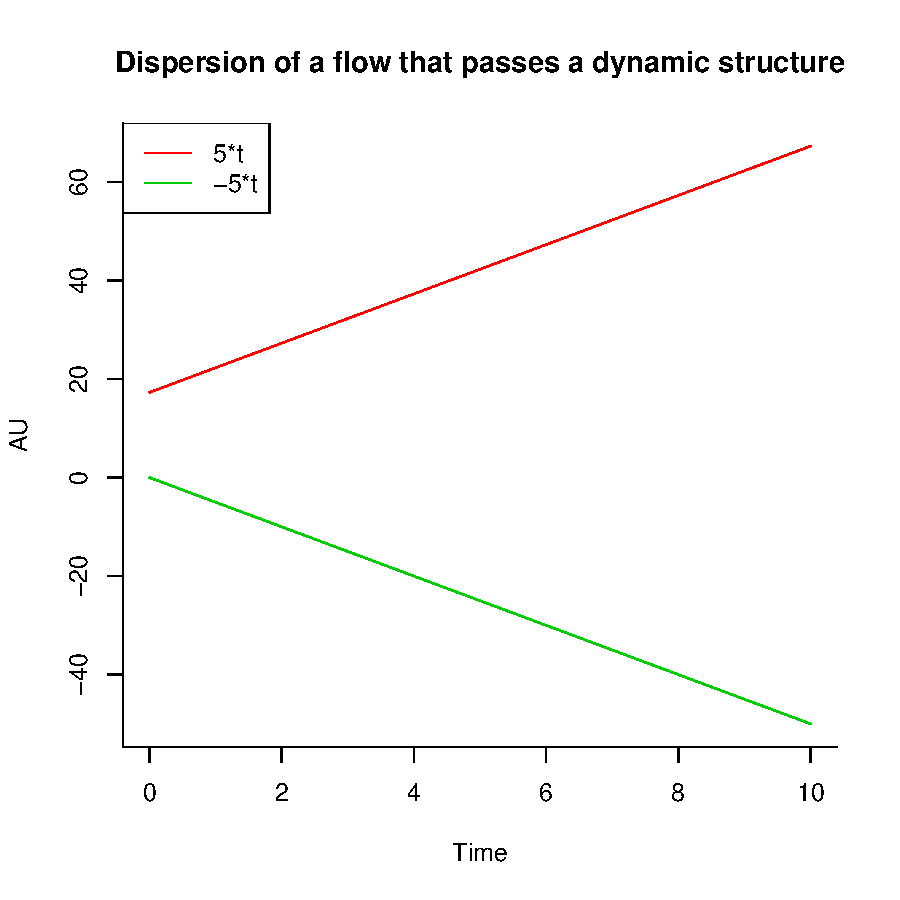
\includegraphics{L1-001}
\pagebreak
\begin{Schunk}
\begin{Sinput}
> ## =============================================================================
> ## 2.2 Possitive feedback
> ## =============================================================================
> rm(list=ls(all=TRUE))
> derivs <- function(time, state, parameters) {
+   with(as.list(c(state, parameters)), {
+     dX1 <- X1/T1
+     dX2 <- X2/T2
+     dX3 <- X3/T3
+     return(list(c(dX1, dX2, dX3)))
+   })
+ }
> init <- c(X1 = 1, X2 = 1, X3 = 1)
> parameters <-  c(T1 = 5, T2 = 10, T3 = 20)
> times <- seq(0, 10, by = 0.01)
> out <- as.data.frame(ode(y = init, times = times,
+                          func = derivs, parms = parameters))
> out$time <- NULL
> ##-----------------------------
> ## Plot results
> ##-----------------------------
> matplot(times, out, type = 'l', xlab = 'Time', ylab = 'AU',
+         main = 'Positive Feedback', lty = 1, bty = 'l', col = 2:4)
> legend('topleft', c('T=5','T=10','T=20'), lty = 1, col = 2:4)
\end{Sinput}
\end{Schunk}
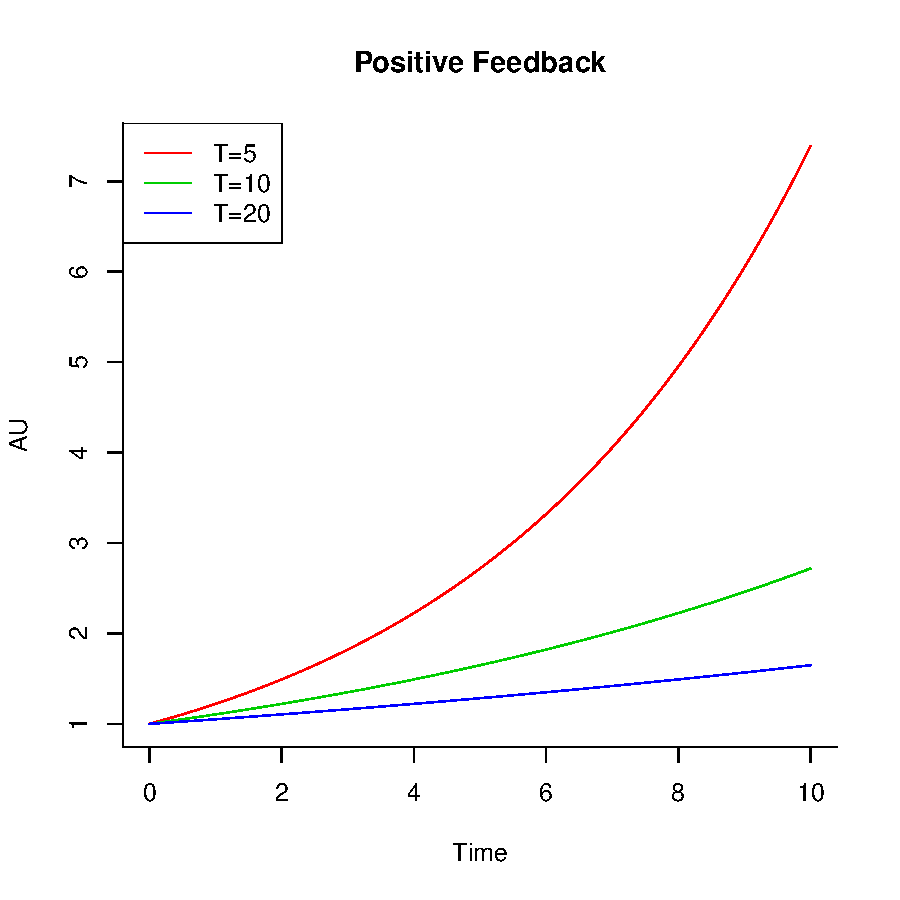
\includegraphics{L1-002}
\pagebreak
\begin{Schunk}
\begin{Sinput}
> ## =============================================================================
> ## 2.3a Negative feedback
> ## =============================================================================
> rm(list=ls(all=TRUE))
> derivs <- function(time, state, parameters) {
+   with(as.list(c(state, parameters)), {
+     dX1 <- -X1/T1
+     dX2 <- -X2/T2
+     dX3 <- -X3/T3
+     return(list(c(dX1, dX2, dX3)))
+   })
+ }
> init <- c(X1 = 100, X2 = 100, X3 = 100)
> parameters <-  c(T1 = 5, T2 = 10, T3 = 20)
> times <- seq(0, 50, by = 0.01)
> out <- as.data.frame(ode(y = init, times = times, 
+                          func = derivs, parms = parameters))
> out$time <- NULL
> ##-----------------------------
> ## Plot results
> ##-----------------------------
> matplot(times, out, type = 'l', xlab = 'Time', ylab = 'AU', 
+         main = 'Negative Feedback', lty = 1, bty = 'l', col = 2:4)
> legend('topright', c('T=5','T=10','T=20'), lty = 1, col = 2:4)
\end{Sinput}
\end{Schunk}
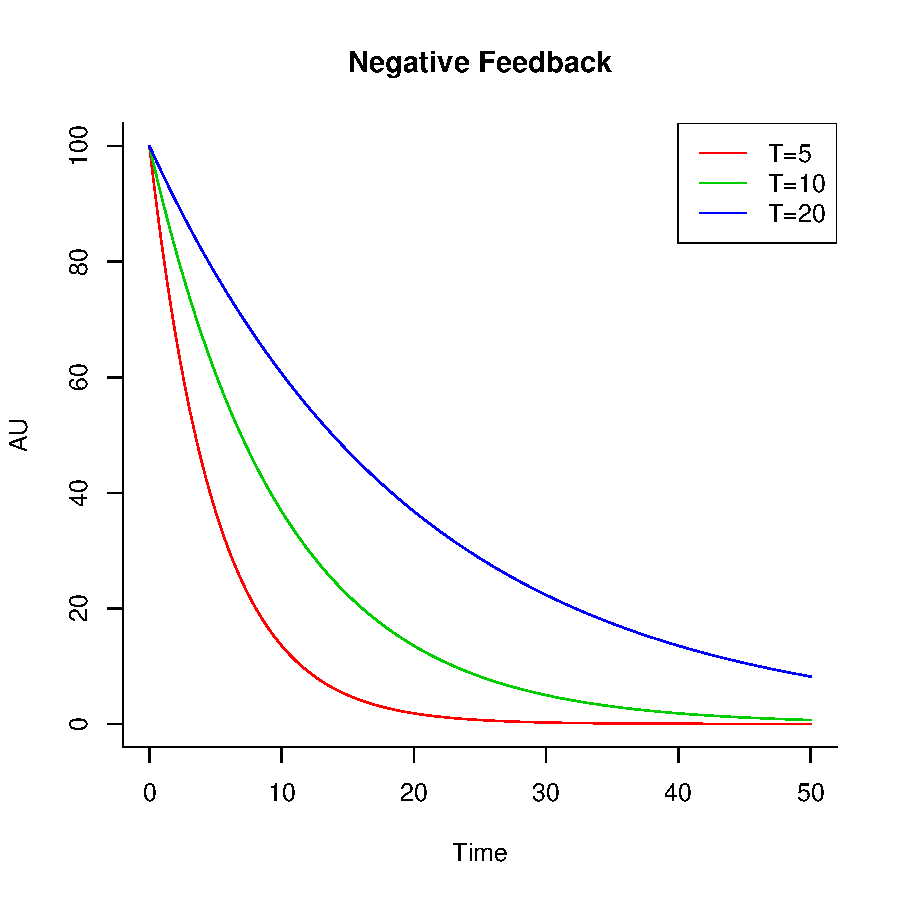
\includegraphics{L1-003}
\pagebreak
\begin{Schunk}
\begin{Sinput}
> ## =============================================================================
> ## 2.3b Avarage Sojurn Time
> ## =============================================================================
> rm(list=ls(all=TRUE))
> derivs <- function(time, state, parameters) {
+   with(as.list(c(state, parameters)), {
+     dX1 <- -X1/T1
+     Av_Time <- -time * dX1 / 100
+     return(list(c(dX1, Av_Time)))
+   })
+ }
> init <- c(X1 = 100, Av_Time = 0)
> parameters <-  c(T1 = 10)
> times <- seq(0, 100, by = 0.01)
> out <- as.data.frame(ode(y = init, times = times, 
+                          func = derivs, parms = parameters))
> out$time <- NULL
> ##-----------------------------
> ## Plot results
> ##-----------------------------
> matplot(times, out, type = 'l', xlab = 'Time', ylab = 'AU', 
+         main = 'Avarage sojourn time', lty = 1, bty = 'l', col = 2:3)
> legend('topright', c('X','Avarage Time'), lty = 1, col = 2:3)
\end{Sinput}
\end{Schunk}
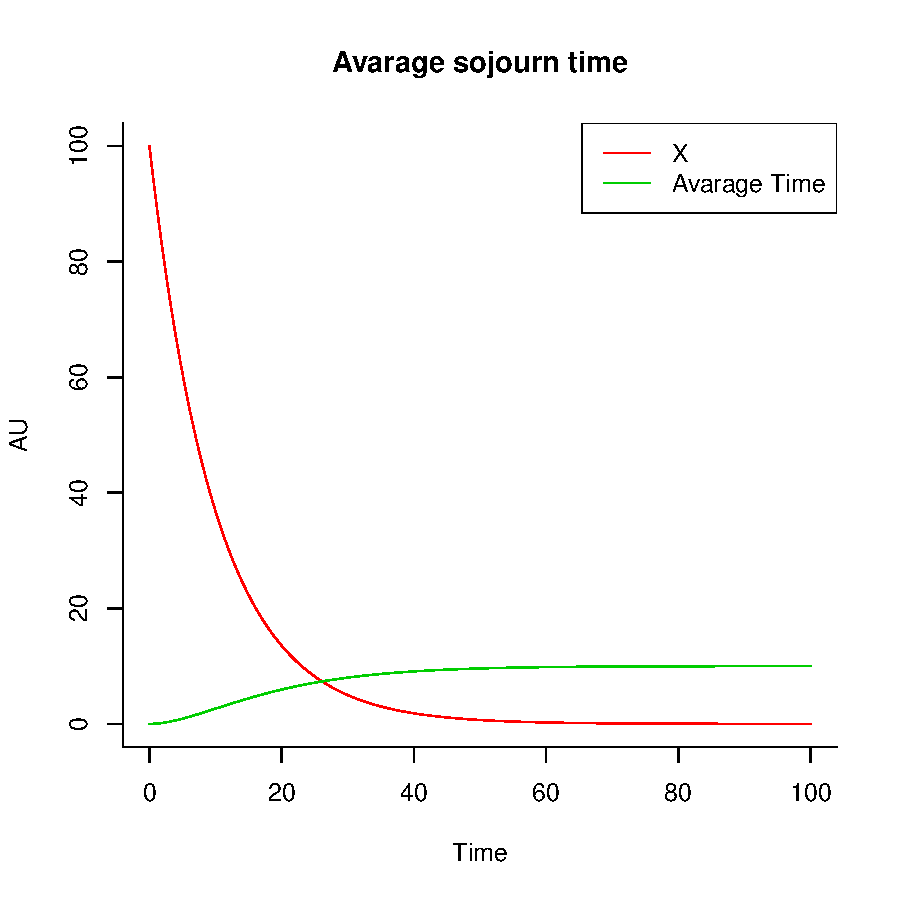
\includegraphics{L1-004}
\pagebreak
\begin{Schunk}
\begin{Sinput}
> ## =============================================================================
> ## 2.4 Negative feedback over two compartments
> ## =============================================================================
> rm(list=ls(all=TRUE)) 
> oscillation <- function(time, state, parameters) {
+   with(as.list(c(state, parameters)), {
+     dX2 <- -X1
+     dX1 <- X2    
+     return(list(c(dX1, dX2)))
+   })
+ }
> init <- c(X1 = 20, X2 = 0)
> parameters <- NULL
> times <- seq(0, 10, by = 0.01)
> out <- as.data.frame(ode(y = init, times = times, 
+                          func = oscillation, parms = parameters))
> out$time <- NULL
> layout(matrix(c(1,1,2,3), 2, 2, byrow = TRUE))
> matplot(times, out, type = "l", xlab = "Time", ylab = "AU",
+         main = "Negative feedback over two compartments", 
+         lwd = 1, lty = 1, bty = "l", col = 2:3)
> plot(out$X1,out$X2, type = 'l',ylab='X2', xlab='X1')
\end{Sinput}
\end{Schunk}
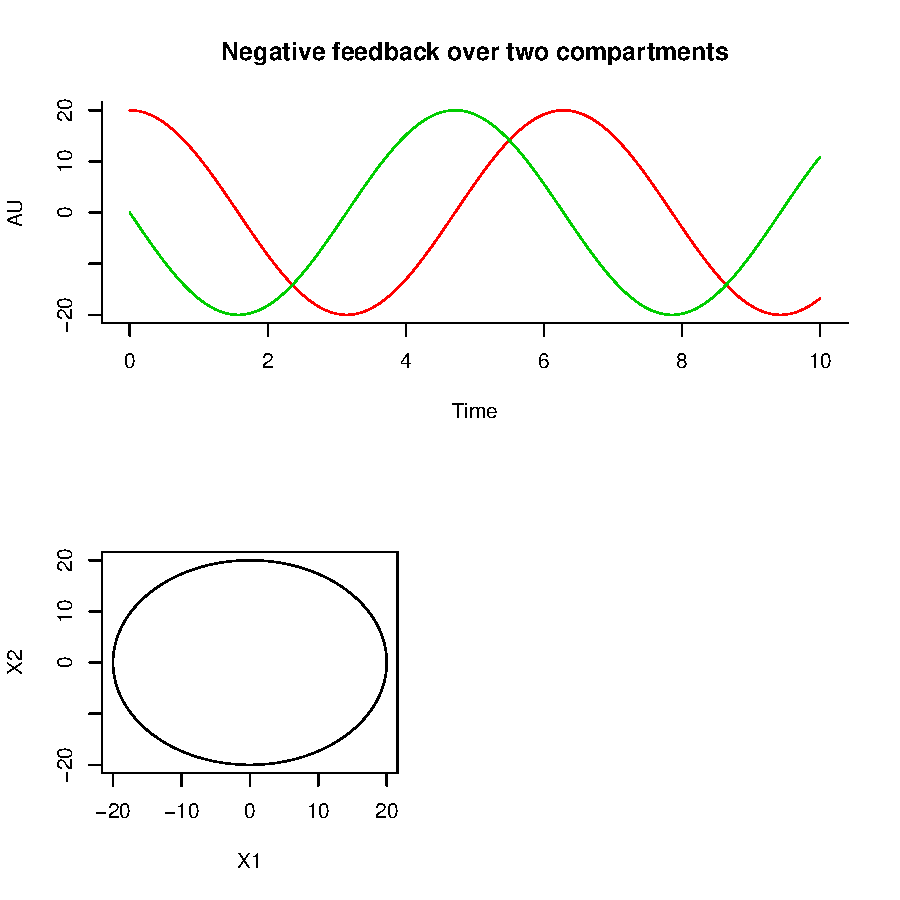
\includegraphics{L1-005}
\pagebreak
\begin{Schunk}
\begin{Sinput}
> ## =============================================================================
> ## 2.5 Dispertion by a dynamic structure
> ## =============================================================================
> rm(list=ls(all=TRUE)) 
> deriv <- function(time, state, parameters) {
+   with(as.list(c(state, parameters)), {
+     import <- sigimp(time)
+     dX1 <- (import - X1)/T0
+     dX2 <- (X1 - X2)/T0
+     dX3 <- (X2 - X3)/T0 
+     return(list(c(dX1, dX2,dX3)))
+   })
+ }
> init <- c(X1 = 0, X2 = 0, X3 = 0)
> parameters <- c(T0=10)
> dt <- 0.01
> times <- seq(0, 100, by = dt)
> ## external signal with triangle impulse with area 100
> signal <- as.data.frame(list(times = times, import = rep(0,length(times))))
> #The 2 since it is a triangle
> signal$import[signal$times >= 0 & signal$times <= 0] <- 100 / dt * 2
> sigimp <- approxfun(signal$times, signal$import, rule = 2)
> out <- as.data.frame(ode(y = init, times = times, 
+                          func = deriv, parms = parameters))
> out$time <- NULL
> ##-----------------------------
> ## Plot results
> ##-----------------------------
> matplot(times, cbind(sigimp(times),out), type = 'l', xlab = 'Time', ylab = 'AU',
+         main = 'Dispersion of a flow that passes a dynamic structure', lwd = 1, 
+         lty = 1, bty = 'l', col = 2:5, ylim=c(0,12))
> legend('topright', c('Pulse','X1', 'X2','X3'), lty = 1, col = 2:5)
\end{Sinput}
\end{Schunk}
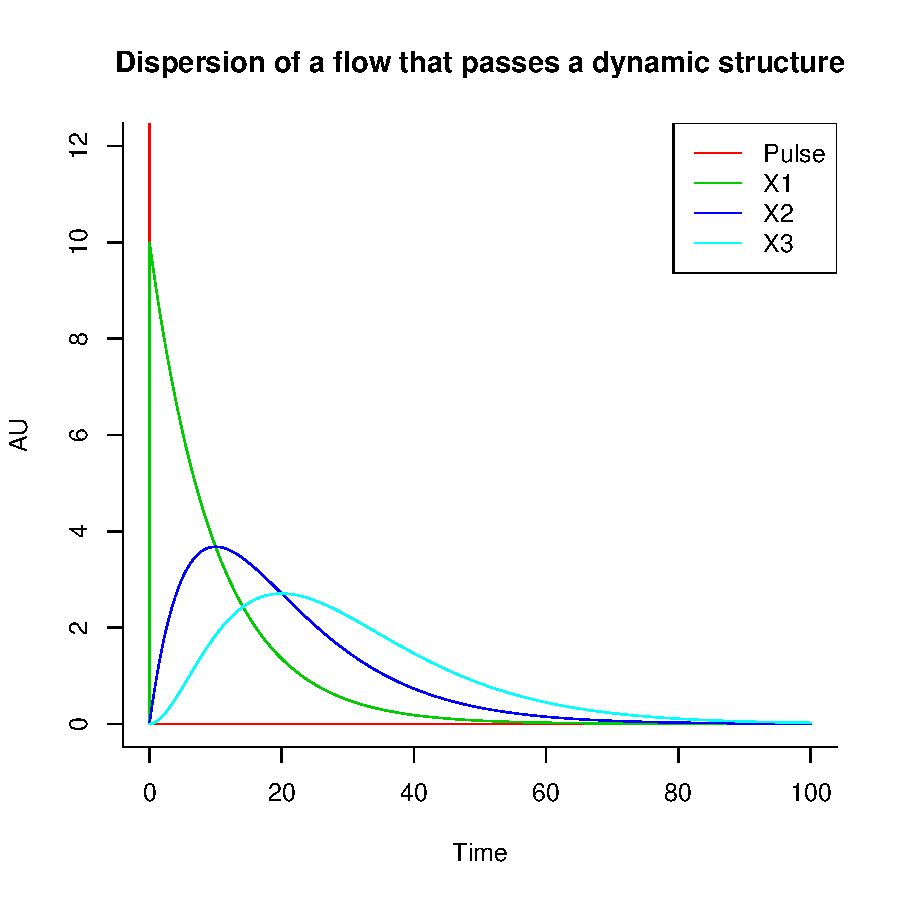
\includegraphics{L1-006}
\pagebreak
\begin{Schunk}
\begin{Sinput}
> ## =============================================================================
> ## 2.6 A logistic and an SI structure
> ## =============================================================================
> rm(list=ls(all=TRUE)) 
> deriv <- function(time, state, parameters) {
+   with(as.list(c(state, parameters)), {
+     dX <- c1 * X - c2 * X * X
+     dS <-   - r * I * S
+     dI <-     r * I * S
+     return(list(c(dX, dS, dI)))
+   })
+ }
> init <- c(X = 1, S=99, I = 1)
> parameters <- c(c1=1, c2=0.01, r=0.01)
> times <- seq(0, 20, by = 0.01)
> out <- as.data.frame(ode(y = init, times = times,
+                          func = deriv, parms = parameters))
> out$time <- NULL
> out$S <- NULL
> ##-----------------------------
> ## Plot results
> ##-----------------------------
> matplot(times, out, type = c('o','l'), xlab = 'Time', ylab = 'AU', 
+         main = 'Logistic Model & SI-model', pch = 1, lwd =4, col = 2:4)
> legend('topleft', c('Logistic Model','SI-model'), 
+        pch = c('o','-'), lwd =c(0,4), col = 2:4)
\end{Sinput}
\end{Schunk}
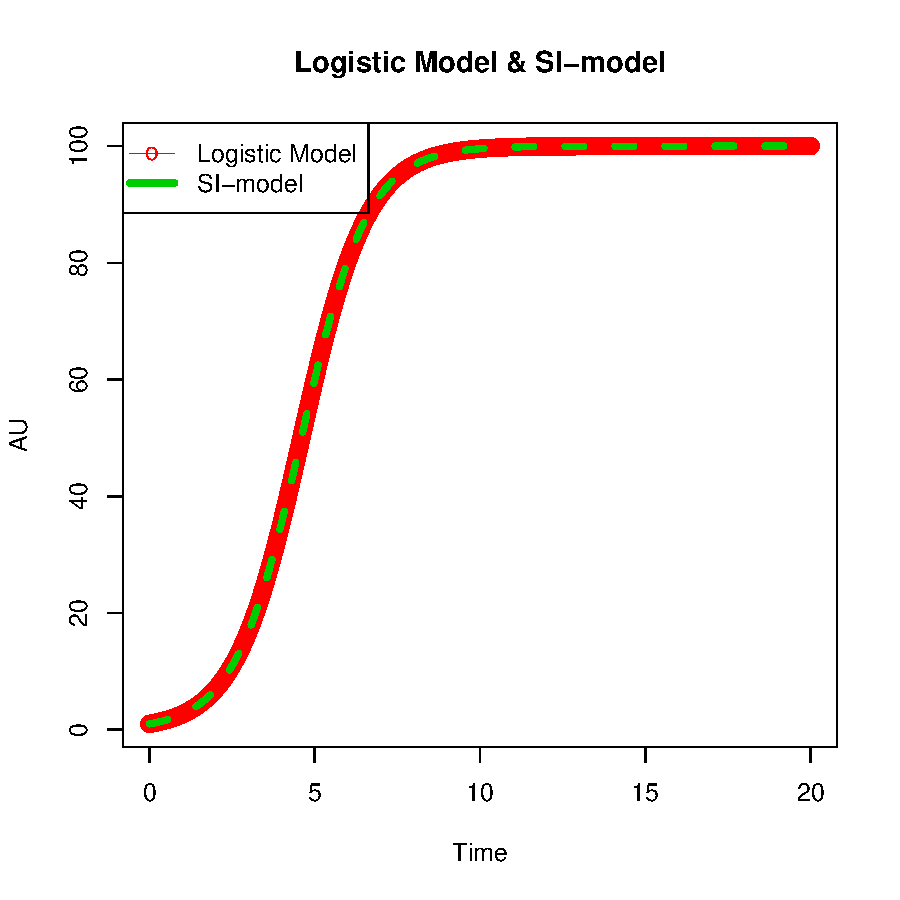
\includegraphics{L1-007}
\pagebreak
\begin{Schunk}
\begin{Sinput}
> ## =============================================================================
> ## 3 Equation behind a Forrester diagram
> ## =============================================================================
> rm(list=ls(all=TRUE)) 
> deriv <- function(time, state, parameters) {
+   with(as.list(c(state, parameters)), {
+     dX <- c1 -X/T1
+     return(list(c(dX)))
+   })
+ }
> init <- c(X = 0)
> parameters <- c(c1=1, T1 = 10)
> times <- seq(0, 100, by = 0.01)
> out <- as.data.frame(ode(y = init, times = times, func = deriv,
+                          parms = parameters, method='euler'))
> out$time <- NULL
> ##-----------------------------
> ## Plot results
> ##-----------------------------
> matplot(times, out, type = 'l', xlab = 'Time', ylab = 'AU',
+         main = 'Logistic Model & SI-model', pch = 1, col = 2)
> legend('topright', c('X'), pch ='-', col = 2)
\end{Sinput}
\end{Schunk}
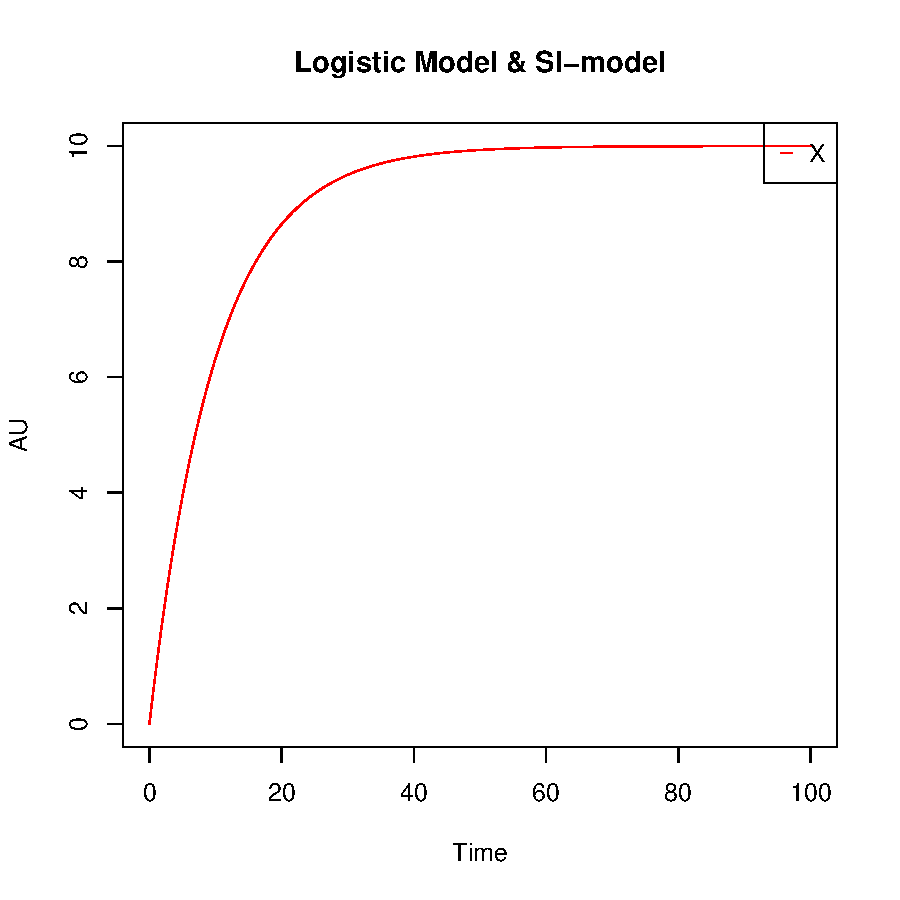
\includegraphics{L1-008}
\pagebreak
\begin{Schunk}
\begin{Sinput}
> ## =============================================================================
> ## 5 Equation behind a Forrester diagram
> ## =============================================================================
> rm(list=ls(all=TRUE)) 
> deriv <- function(time, state, parameters) {
+   with(as.list(c(state, parameters)), {
+     dX <- c1 -X/T1
+     return(list(c(dX)))
+   })
+ }
> init <- c(X = 0)
> parameters <- c(c1=1, T1 = 10)
> d_t <- c(5, 2, 0.1, 0.01)
> for (tt in 1:length(d_t)){
+   times <- seq(0, 100, by = d_t[tt])
+   out <- as.data.frame(ode(y = init, times = times, func = deriv, 
+                            parms = parameters, method='euler'))
+   out$time <- NULL
+   if (tt==1)
+     matplot(times, out, type = 'l', xlab = 'Time', ylab = 'AU', 
+             main = 'Choosing time-step', pch = 1, col = 1)
+   else
+     lines(times, t(out), col = tt)
+ }
> legend('topright', sprintf("dt=%.2f", d_t), pch ='-', col = (1:(length(d_t))))
\end{Sinput}
\end{Schunk}
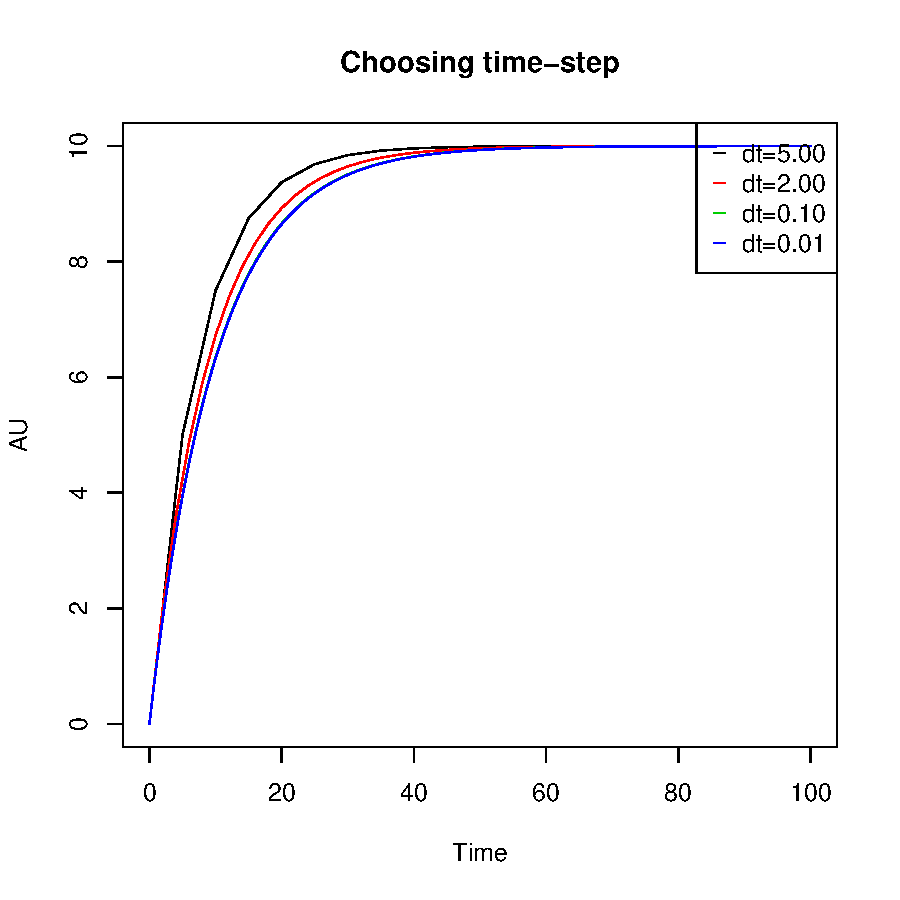
\includegraphics{L1-009}
\pagebreak
\begin{Schunk}
\begin{Sinput}
> ## =============================================================================
> ## 6 Stage and Compartment
> ## =============================================================================
> rm(list=ls(all=TRUE)) 
> deriv <- function(time, state, parameters) {
+   with(as.list(c(state, parameters)), {
+     import <- sigimp(time)
+     # One compartment
+     dX1   <- (import - X1)/T1
+     # Two compartments
+     dX2_1 <- (import - X2_1)/T2
+     dX2_2 <- (X2_1 - X2_2)/T2
+     # Three compartments
+     dX3_1 <- (import - X3_1)/T3
+     dX3_2 <- (X3_1 - X3_2)/T3
+     dX3_3 <- (X3_2 - X3_3)/T3 
+     return(list(c(dX1, dX2_1, dX2_2, dX3_1, dX3_2, dX3_3)))
+   })
+ }
> init <- c(X1 = 0, X2_1 = 0, X2_2 = 0, X3_1 = 0, X3_2 = 0, X3_3 = 0)
> parameters <- c(T1 = 10, T2 = 10/2, T3 = 10/3)
> d_t <- 0.01
> times <- seq(0, 100, by = d_t)
> ## external signal with triangle impulse with area 1
> signal <- as.data.frame(list(times = times, import = rep(0,length(times))))
> #The 2 since it is a triangle
> signal$import[signal$times >= 0 & signal$times <= 0] <- 1 / d_t * 2
> sigimp <- approxfun(signal$times, signal$import, rule = 2)
> out <- as.data.frame(ode(y = init, times = times, func = deriv, parms = parameters))
> ##-----------------------------
> ## Plot results
> ##-----------------------------
> matplot(times, out[c('X1','X2_2','X3_3')], type = 'l', xlab = 'Time', ylab = 'AU', 
+         main = 'Multiple compartments', lwd = 1,
+         lty = 1, bty = 'l', col = 2:5, ylim=c(0,0.1))
> legend('topright', c('1 Compartment', '2 Compartments','3 Compartments'),
+        lty = 1, col = 2:5)
\end{Sinput}
\end{Schunk}
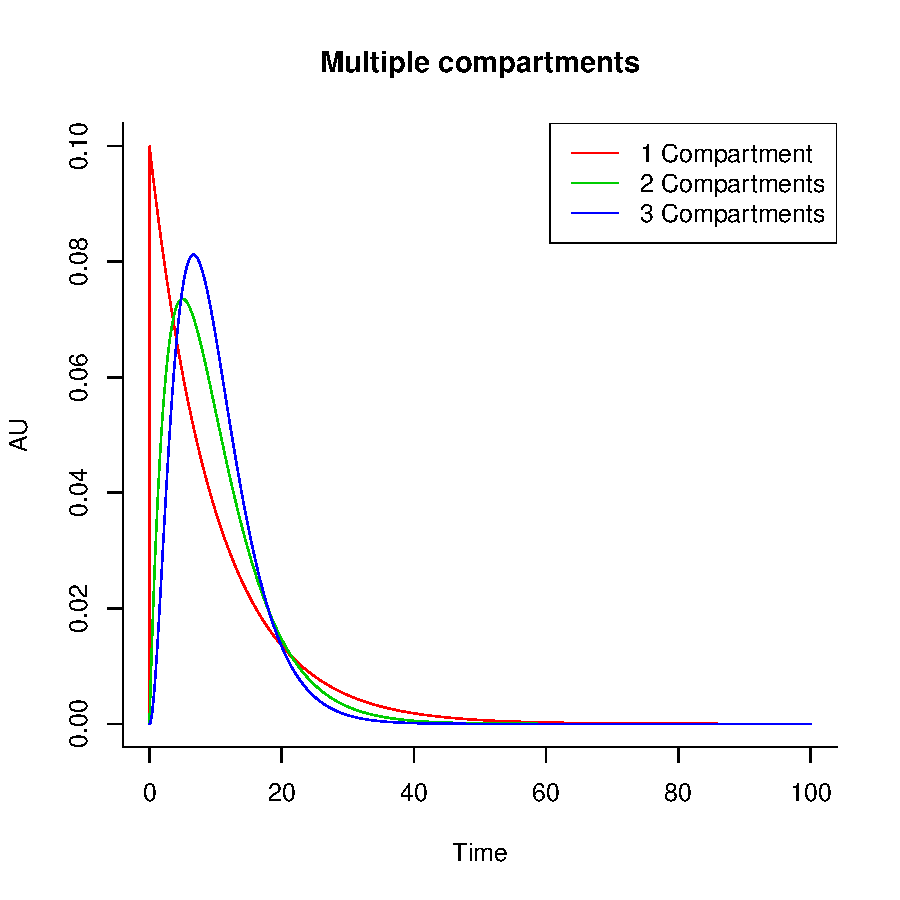
\includegraphics{L1-010}

\end{document}
